\documentclass[a4paper,20pt]{article}
\usepackage{amsmath}
\usepackage{amssymb}
%\usepackage[a4paper, total={15cm, 20cm}]{geometry}
\usepackage{graphicx}
\usepackage{hyperref}
\usepackage{indentfirst}
\hypersetup{colorlinks=true, linkcolor=blue}

%% Documents settings
\title{Projet Optimisation}
\author{Vasavan \& Wesley}

\begin{document}
%% Generate the title
\maketitle
\newpage
\protect\hypertarget{table}{}
\renewcommand{\contentsname}{Sommaire}
\tableofcontents
\newpage
\newpage

\section{Objectif}
La mission d'un lanceur spatial est d'amener un satellite en orbite. Le
 probl\`eme est divis\'e en deux parties l'impl\'ementation de l'algorithme SQP
 (Sequential Quadratic Programming) et l'impl\'ementation d'un simulateur, le
 tout en \textit{Matlab}.
\newpage

\section{Algorithme et logiciel}
\subsection{Optimisateur SQP}
L'algorithme SQP permet de r\'esoudre des probl\`emes non lin\'eaires sous
 contraintes.

\begin{figure}[h!]
\centering
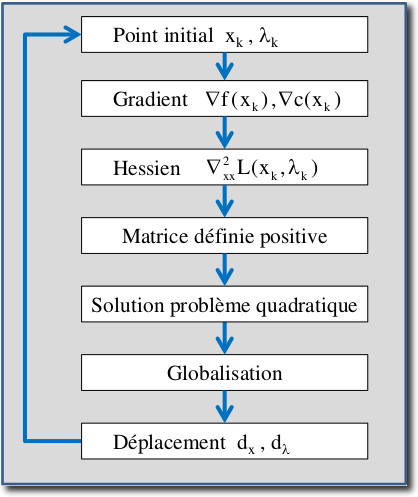
\includegraphics[width=6cm]{capture.png}
\caption{Organigramme}
\label{fig:1}
\end{figure}

\subsection{Calcul du gradient}
Le calcul du gradient de la fonction co\^ut f et de
la fonction contrainte est fait par la méthode des diff\'erences finies.

\subsection{Calcul du hessien}
Le calcul du hessien est fait par une m\'ethode de Quasi-Newton. Les
 it\'erations sur le hessien sont faites soit par la méthode BFGS ou soit par la
 méthode SR1.

\subsection{Probl\`eme quadratique}
Cette partie r\'esolve le probl\`eme quadratique en prenant en argument la
 matrice hesienne d\'efinie positive, les gradients des fontcions co\^ut f et de
 la fonction contrainte.

\subsection{Globalisation}
Cette partie est compos\'e de plusieurs \'etapes. On v\'erifie tout d'abord que
 la fonction de m\'erite est d\'ecroissante, si elle ne l'est pas on
 r\'einitialise le Hessien, puis on recherche une direction de d\'escente en
 augmentant $\rho$.

\section{Test de validation de l'optimiseur SQP}
Plusieurs cas test sont effectu\'es pour valider l'optimiseur SQP. Les cas test
 sont : MHW4D et Ariane.


\subsection {Cas test: MHW4D}
Le probl\`eme:
$$
\begin{cases}
\min\limits_{x\in\mathbb{R}^3}{(x_1-1)^2+(x_1-x_2)^2+(x_2-x_3)^3+(x_3-x_4)^4
+(x_4-x_5)^4} \\
x_1+x_2^2+x_3^2-3\sqrt{2}-2=0 \\
x_2+x_3^2+x_4-2\sqrt{2}+2=0 \\
x_1x_5-2=0
\end{cases}
$$

Tableau des valeurs initiales

Tableau des valeurs finales

\subsection{Cas test: Ariane}
Les masses:
\begin{align*}
m_u &= 1700 & & & & & & \\
K &= (0.1101, 0.1532, 0.2154) & & & & & & \\
V_e &= (2647.2, 2922.4, 4344.3) & & & & & & \\
M_s &= (K_1M_{e,1}, K_2M_{e,2}, K_3M_{e,3}) & & & & & & \\
\end{align*}
\begin{align*}
M_{i,1} &= m_u &+ M_{s,3} &+ M_{e,3} &+ M_{s,2} &+ M_{e,2} &+ M_{s,1} &+ M_{e,1}
 \\
M_{f,1} &= m_u &+ M_{s,3} &+ M_{e,3} &+ M_{s,2} &+ M_{e,2} &+ M_{s,1} & \\
M_{i,2} &= m_u &+ M_{s,3} &+ M_{e,3} &+ M_{s,2} &+ M_{e,2} & & \\
M_{f,2} &= m_u &+ M_{s,3} &+ M_{e,3} &+ M_{s,2} & & & \\
M_{i,3} &= m_u &+ M_{s,3} &+ M_{e,3} & & & & \\
M_{f,3} &= m_u &+ M_{s,3} & & & & & \\
\end{align*}
Le probl\`eme:
\begin{equation*}
\begin{cases}
\min\limits_{m_e\in\mathbb{R}^3}{m_{e,1}+m_{s,1}+m_{e,2}+m_{s,2}+m_{e,3}+m_{s,3}
+m_u} \\
V_{e,1}\ln\left(\frac{M_{i,1}}{M_{f,1}}\right)
+V_{e,2}\ln\left(\frac{M_{i,2}}{M_{f,2}}\right)
+V_{e,3}\ln\left(\frac{M_{i,3}}{M_{f,3}}\right)-11527=0
\end{cases}
\end{equation*}

Tableau des valeurs:
$$
\begin{array}{|c|c|c|c|}
\hline
\text{It\'eration} & \text{Masses} & \text{Lambda} & \text{Norme du lagrangien} \\
\hline
1 & (177362.639639, 47615.194077, 10000.00000) & 346820.596063 & 10745.501622 \\
2 & (148052.357121, 29654.350488, 10000.00000) & 3786571979.219226 & 117330866.704092 \\
2 & (148052.357121, 29654.350488, 10000.00000) & 798735300.897798 & 7499814.214797 \\
3 & (148088.338651, 29703.590875, 9946.238284) &-3666278.867516 & 81537.247633 \\
4 & (148088.625409, 29703.982835, 9945.812910) &-60590.677561 & 1347.261577 \\
5 & (148088.634574, 29703.995365, 9945.799295) &-26.034761 & 2.006907 \\
6 & (148088.634574, 29703.995365, 9945.799295) &-17.909327 & 1.990368 \\
7 & (148088.631890, 29703.991781, 9945.802594) &-17.908987 & 1.990366 \\
8 & (148088.631890, 29703.991781, 9945.802594) &238.639221 & 5.860333 \\
9 & (148088.630906, 29703.990798, 9945.801174) &-13.499187 & 1.988031 \\
10 & (148088.630905, 29703.990798, 9945.801173) &417.741349 & 9.636206 \\
11 & (148088.630905, 29703.990798, 9945.801173) &-16.561310 & 1.989155 \\
12 & (148088.630905, 29703.990798, 9945.801173) &-16.561310 & 1.989154 \\
\hline
\end{array}
$$

\section{Lanceur spatial}
La simulation du lanceur spatial est divis\'e en deux parties majeures : le
 probl\`eme d'\'etagement et le probl\`eme de trajectoire.

\subsection{Probl\`eme d'\'etagement}
Le probl\`eme d'\'etagement est un probl\`eme d'optimisation des masses
 d'\'ergols de la fus\'ee. Il est r\'esolu par l'optimiseur SQP.

1.4.1) On reformule le probl\`eme. Avec $x_j=\frac{M_{i,j}}{M_{f,j}}$
$$
J=\frac{M_{i,4}}{M_{i,3}}\cdot\frac{M_{i,3}}{M_{i,2}}
\cdot\frac{M_{i,2}}{M_{i,1}}=\prod\limits_{j=1}^3\frac{M_{i,j+1}}{M_{i,j}} \\
$$
\begin{equation*}
\begin{split}
\frac{M_{i,j+1}}{M_{i,j}}&=1-(k_j+1)(1-x_j^{-1}) \\
&=\frac{-x_jk_j+k_j+1}{x_j} \\
&=-\left[\frac{1+k_j}{x_j}-k_j\right]
\end{split}
\end{equation*}
Ainsi:
$$
f(x)=-\prod\limits_{j=1}^3\left(\frac{1+k_j}{x_j}-k_j\right)
$$
La condition KKT est en $x=(x_1, x_2, x_3)$:
$$
\nabla f+\nabla c\lambda=0
$$
Soit pour $j\in\{1, 2, 3\}$:
$$
\frac{\partial f}{\partial x_j}+\lambda\frac{\partial c}{\partial x_j}=0
$$
$$
\left(\frac{1+k_j}{x_j^2}\right)\prod\limits_{i=1, i\neq j}^3
\left(\frac{1+k_i}{x_i}-k_i\right)+\lambda\frac{v_j}{x_j}=0
$$
$$
\lambda=\frac{-1}{v_j}\cdot\frac{1+k_j}{k_jx_j}
\cdot\prod\limits_{i=1, i\neq j}^3\left(\frac{1+k_j}{k_jx_j}-1\right)
$$
On obtient finalement:
$$
\begin{cases}
v_2(1-\Omega_2x_2)&=v_1(1-\Omega_1x1) \\
v_2(1-\Omega_2x_2)&=v_3(3-\Omega_3x3)
\end{cases}
$$
\subsection{Probl\`eme de trajectoire}
La trajectoire du lanceur est d\'ecoup\'ee en trois s\'equences correspondant au
 fonctionnement successif des trois \'etages propulsifs. La simulation de la
 trajectoire est mod\'elis\'ee par des \'equations de Mouvements que l'on
 r\'esout par int\'egration num\'erique, en utilisant la fonction ODE45 de
 Matlab.

\subsection{Optimisation des angles}
Pour avoir une trajectoire optimis\'ee, on r\'esout finalement le probl\`eme
 suivant sur les angles, en utilisant l'algorithme SQP :

\section{Simulation du lanceur}
\subsection{Visualisation}
\begin{figure}[h!]
\centering
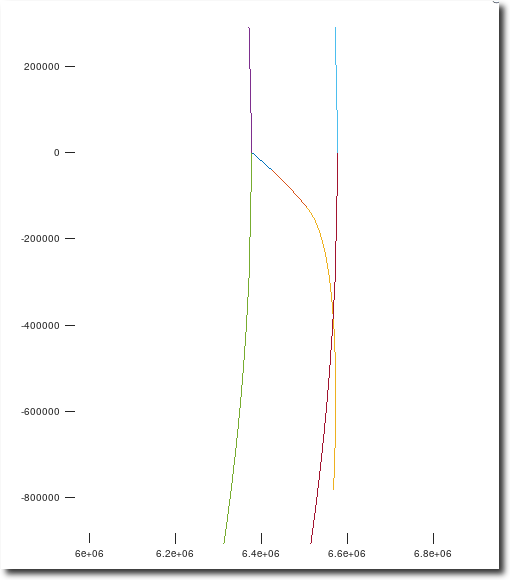
\includegraphics[width=6cm]{trajectoire.png}
\caption{Trajectoire}
\label{fig:1}
\end{figure}

% Capture la trajection non-optimiser (image), tableau, ..., excuse
\section{Probl\`emes et limites rencontr\'es}
% Optimisation non reussie, probleme (histoire des bugs)

Nous avons rencontrés des difficultés dans l'optimisation des thétas. Ce qui nous a pas permis d'aboutir le projet correctement.

\end{document}
